\chapter{Literature Review}
The literature review is aggregated with three sections, covering topics Chinese character recognition \& generation, neural networks and mathematical morphology respectively, which are highly connected with our project as background technical information.

\section{Chinese Character Recognition \& Generation}
When it comes to automatic recognition or generation of actual oracle bone scripts, there are very limited resources. Most of them still work on establishment of fundamental computer tools for research, Shi et al.\cite{Shi2005} digitalised scanning photos of oracle bone scripts, turning them into vector graphs in .svg format for web use; Liu et al.\cite{Liu2004} wrote a Visual C++ application on Windows as visual input method for oracle bone script characters. And when we turned ourselves to modern Chinese character recognition and hope that such researches can guide us to a correct track, a lot of relative papers were found. Previous work on Chinese character recognition based on neural networks was mainly in handwritten character, which was considered as a difficult task generally. In 2010, Chinese handwriting recognition contest\cite{5659229} showed that for GB2312-80 level-1 set, the most frequently-used modern Chinese character set in mainland China, off-line recognition accuracy of the top system (HKU) reached only 89.99\%, let alone oracle bone scripts which has no standard uniform glyphs decided by academia.

Based on these facts, Xue et al.\cite{xue2014recognition} decided to improve accuracy by distinguish between easily confused Chinese characters; authors combined character feature extraction and feature dimension reduction together, providing a new CNN-based similar character recognition system. Xu et al.\cite{xu2008automatic} proposed a method which trains machine to learn calligraphic handwriting style of a specific writer. And Xu et al.\cite{1439477} also invented an algorithm that enables the computer to generate Chinese calligraphic handwritings with special aesthetic requirements learnt from training samples.

In \cite{7327196}, authors collected a dataset called Oracle-20K from Chinese Etymology\footnote{\url{http://hanziyuan.net}, which is also one of our data sources.}, a data set of sketching objects distributed over 250 different categories, and claimed that their dataset was the largest oracle character dataset in computer vision so far, although they did not actually release it. To build the dataset, they removed all glyphs which contain less than 25 unique samples and eleven low-level representations in total and four mid-levels ones (based on multi-layer sparse autoencoder) were used to represent oracle bone scripts.

Eventually, Liu et al.\cite{6376394} introduced a unique approach to generate personal handwriting style for Chinese characters, which is quite close to what we planned to do. First a Chinese character is split into parts represented quantitatively by multi-dimensional vectors, ``such as strokes, radicals and frequent character components''. After analysing on topological structure of the whole character and spatial relationships between each component, authors put forward a representation ``parameterising the character's topological structure, its layout, as well as the relative length distribution of two strokes''. And later on an overall similarity between two components can be calculated, used in handwriting facsimile.

\section{Neural Networks}
Neural network, also referred as artificial neural network, a computational model which is a vaguely simplified version of biological neural networks, consisting of animal brains. Neural networks constitutes a set of connected nodes called neurons, a mathematical function that sums up all weighed inputs (signals) from other neurons and applies an activation function on it as outputs. And activation functions used in neurons are often non-linear like logistic functions, or rectified linear (ReLU) function. And connections are referred as edges in neural network context. The weight changes by back propagation and sometimes neurons may have a threshold to decide if the signal is sent or not. Typically neurons are divided into multiple layers and different layers apply different types of transformations.

\subsection{Convolutional Neural Networks}
Nowadays, convolutional neural network (CNN or ConvNet) is considered as a prevalent model for image classification. This model resembles original neural networks with ``learnable'' weights and biases, applying loss function (like SoftMax function that we used in our project) to last layer. It is a type of multilayer perceptrons with several levels of hidden layers, including convolutional layers, pooling layers and finally, fully connected layers.

CNN can result in high accuracy rates, even better than human performance in some cases like MNIST recognition. Besides, CNN becomes very efficient by using filters. ``CNNs have much fewer connections and parameters and so they are easier to train''\cite{Krizhevsky:2012:ICD:2999134.2999257}, and involves relatively not intensive preprocessing. In CNN, every single neuron represents a small part of the vision of an image (local receptive field), and all neurons cover all the information in a single image.

\subsection{Generative Adversarial Nets}
To elaborate GANs, we have to go through briefly details on generative model and its counterpart discriminative model from mathematics first. In statistics and probability, a generative model is a statistical model about generation of sample or similar data from a larger population and it learns the joint probability distribution $ P(X, Y) $ and given the same arbitrary input $ X $, conditional probability of $ Y $ can be calculated, $ P(Y | X) $, which a discriminative model can learn from. And for instance, in binary classification problems, if output $ Y $ is greater than some pre-set threshold $ Z $, $ X $ belongs to group $ W_1 $; otherwise, $ X $ is in group $ W_2 $.

And the ultimate task of supervised learning is to build a model (classifier) learned from bulks of data. Therefore, generative adversarial nets is proposed by Ian Goodfellow in 2014\cite{goodfellow2014generative} and offers a new method of deep learning representations without plenty of labelled data. Obviously, GAN is not the only way to apply neural networks in unsupervised learning; auto encoder\cite[ch.~14]{Goodfellow-et-al-2016} and Boltzmann machine\cite[ch.~20]{Goodfellow-et-al-2016}. Previously, two of them worked on extracting features from the equation $ f(x) = x $ and train and generate samples relying on Markov chain and approximate inference\cite[ch.~20]{Goodfellow-et-al-2016}, which are really calculation-consuming; GAN copes with this issue and is not limited to several Markov-suitable probability distribution.

GAN derived from two-player game in game theory and two players are generative model $ G $ and discriminative model $ D $ respectively. Model $ G $ captures data distribution, using data whose noise subjects to uniform / normal distribution to a generate similar real training sample. For this sample itself, it should try it utmost to resemble the real one. In the meantime, discriminative model $ D $ is a binary classifier (which returns probability values) that judges if a sample comes from the training set rather than $ G $. During the whole training process, one side is fixed and the other's network weight is keeping updating and vice versa. Via back propagation, two networks update separately and ``compete'' each other, by optimising their networks simultaneously until reaching Nash equilibrium. At that time, generative model $ G $ subjects to distribution of training data, which indicates that it generates identical data. And discriminative model $ D $ cannot distinguish at all, whose accuracy is around 50\%.
\begin{figure}[h]
	\centering
	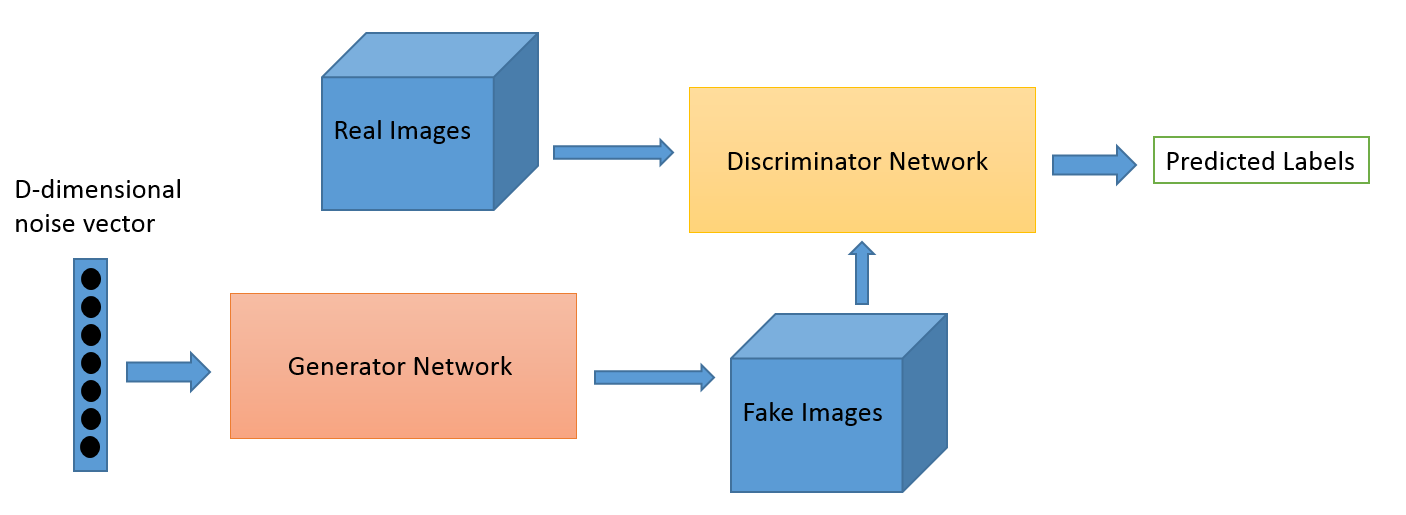
\includegraphics[width=\linewidth]{GAN_Schema.png}
	\caption{General GAN structure (Credit: O'Reilly)}
\end{figure}
And the whole process can be summarised in mathematical fashion as a minimax two-player game:
\[ \underset{G}{\min}\,{\underset{D}{\max}\,V(D, G)={\mathbb{E}_{x\sim{p_{data}(x)}}[\log{D(x)}]+\mathbb{E}_{z\sim{p_{z}(z)}}[\log{(1-D(G(z)))}]}} \]

And this seem-to-be-simple model is vital in the whole history of machine learning. While massive data is available, such as images, voice recordings or plain texts, generative models help us simulate the distribution of these high-dimensional data, which is very futile in many applications. On the other hand, for situation where data is difficult to collect, generative models can create a huge amount of high-quality data and improve efficiency of semi-supervised learning; basically, the whole field of data augmentation is based on it. Specifically, adversarial training can change how we teach AI to fulfil complicated tasks. And in some aspects, these programs learn to become human experts in such a domain.

Although GANs offer us a novel insight into dealing with complex problems, which introduces game theory into machine learning and has extensive impacts, it still has plenty of issues needed to be solved. First and foremost, at least in image generation field, it is not easy to tell how much better GAN is compared to other image generation methods like variational auto-encoder (VAE) or Bayesian networks. It is even harder to prove which one is more efficient: GAN or its derived algorithms. Pitifully, there is not an objective well-accepted standard to gauge difference of various image generation methods; it is inevitably difficult even for human since we judge the genuineness of one image from a few aspects including clearness, object edge colour and appearance of anti-intuitive objects. Only with a reasonable measure method, GAN can be improved systematically.

In GAN, the pictures mapped from the input images to output images domain may have a lot of possibilities which all satisfy the distribution of the output images domain and collapse problem exists. Therefore, researchers\cite{DBLP:journals/corr/ZhuPIE17} proposed CycleGAN (Cycle-Consistent Adversarial Networks) which solved this problem by adding a reverse mapping cycle to enhance the limitations of the conversion. Besides, 70\% of oracle bone scripts do not have paired recognised characters, while CycleGAN is a solution for unpaired image-to-image translation. However, both concluded that it often successes when changing colour and texture of objects. But the task barely succeeds when it requires geometric change, for example, changing a cat to a dog. This happened because the generator architecture is designed for appearance changes.

And the CGAN (Conditional GAN)\cite{DBLP:journals/corr/MirzaO14} is from famous Stanford Computer Vision Lab and it is the first time to come up an idea that adds limitations on GAN to increase accuracy since images generated from original GAN are largely vague in practice. Although the improvement was considered as ``straightforward'', it was highly effectively:
\[ \underset{G}{\min}\,{\underset{D}{\max}\,V(D, G)={\mathbb{E}_{x\sim{p_{data}(x)}}[\log{D(x \mid y)}]+\mathbb{E}_{z\sim{p_{z}(z)}}[\log{(1-D(G(z \mid y)))}]}} \]
Data are labelled in both generative and discriminative models and according to authors' experiments, new generated images contains far more textures.

And the model structure in Pix2Pix\cite{DBLP:journals/corr/IsolaZZE16} resembles work of CGAN. Pairs of same-size pictures are combined as inputs, which changes from three colour channels (RGB) to six ones (which merges two images together), and also $ D(X) $ is replaced by $ D(X, Y) $. And generator $ G $ first encodes input image $ X $ in vector form and decodes to generate image $ Y $. In order to guarantee the high similarity between output image and target one, L1 loss is introduced and makes generated images sharp to a huge extent. And U-Net, closed to residual network, is also used in the paper to merge convoluional kernels from original images to generated ones and reduce much calculation. Noticeably, Pix2Pix introduced a trick called patch, used in Nvidia HD image generation\cite{DBLP:journals/corr/abs-1711-11585}; all images are fed as inputs in partitioned \textbf{patches} form rather than complete images, wherever in generators or discriminators.

\section{Mathematical Morphology}
According to Oxford English Dictionary, morphology, a word borrowed from biology, originally means a study or research of ``the form and structure of animals and plants''. And mathematical morphology (MM) is a framework for image processing based on lattice theory, random geometry\cite{serra1983image} and set theory and is a useful tool for inspecting geometric structures in images\cite{soille2013morphological}. MM ``tends to simplify image data preserving their essential shape characteristics and eliminating irrelevancies''\cite{haralick1987image}, which is suitable for our case since pixel reduction will dramatically speed up tensor-related operations. In this section, a brief introduction mainly highlights structuring element and four basic operators of MM, which are used as thinning algorithm in our code partly.

When a morphological transformation is applied, two inputs are needed: the original image and the SE which decides the nature of operation. The structuring element (SE) is in essence a pre-defined binary shape or template considered as masks normally in matrix form that goes through the image, modifies the pixels based on its ``surrounding neighbours'' it in different methods, providing a huge range of effects on the whole image. It is ``applied to interact with the image to get the resultant''\cite{ravi2013morphological}. The structuring element is therefore typically smaller than the whole image with odd size, not only in number of pixels (or area in the continuous case), but the pixels are also close to each other. ``Size of the structuring element, acts as a 'window' over which the interaction takes place''\cite{ravi2013morphological}. and they ``slide over the image and transform it''. According to \cite{ravi2013morphological}, the structuring element is ``positioned at all possible locations in the image and it is compared with the corresponding neighbourhood of pixels''. Operations on binary images create a new binary ones.

And let $ E $ be a Euclidean space, and $ A $ and $ B $ are binary images in $ E $. And basic operators in MM are listed as followed:
\begin{itemize}
	\item \textbf{Erosion} A method to remove the pixels of foreground edges; it can be represented as $ A \ominus B = \{z \in E \mid B_z \subseteq A\} = \displaystyle \bigcap_{b \in B}^{}A_{-b} $.
	\item \textbf{Dilation} It is just opposite of erosion and enlarges boundaries of foreground area and formal mathematical notion is $ A\oplus B=\bigcup_{b\in B}^{} A_b $.
	\item \textbf{Opening} A method to remove edges of foreground in a less destructive way and the definition is $ A \circ B = (A \ominus B) \oplus B = \displaystyle \bigcup_{B_x\subseteq A}^{} B_x $.
	\item \textbf{Closing} An opposite method to opening tends to extend image area, which is defined as $ A \circ B = (A \oplus B) \ominus B $.
\end{itemize}